\chapter{Related Work}
\label{ch:relatedwork}
\section{網路切片與意圖驅動管理之核心概念}


\subsection{跨網域切片協作之運作機制}

端到端（End-to-End, E2E）網路切片之實作核心在於無線存取網路（RAN）、傳輸網路（TN）與核心網（Core）三大網域間的緊密協作，以在共享之基礎設施上提供具備特定服務等級協議（SLA）保障之邏輯網路 \cite{tran2024ina}。根據 3GPP TS 28.530 規範，一個完整之網路切片實例（Network Slice Instance, NSI）通常由多個網路切片子網實例（Network Slice Subnet Instance, NSSI）構成，分別對應 Core、RAN 與 TN 之資源範疇 \cite{3gpp_ts28530}。

\begin{figure}[H]
\centering
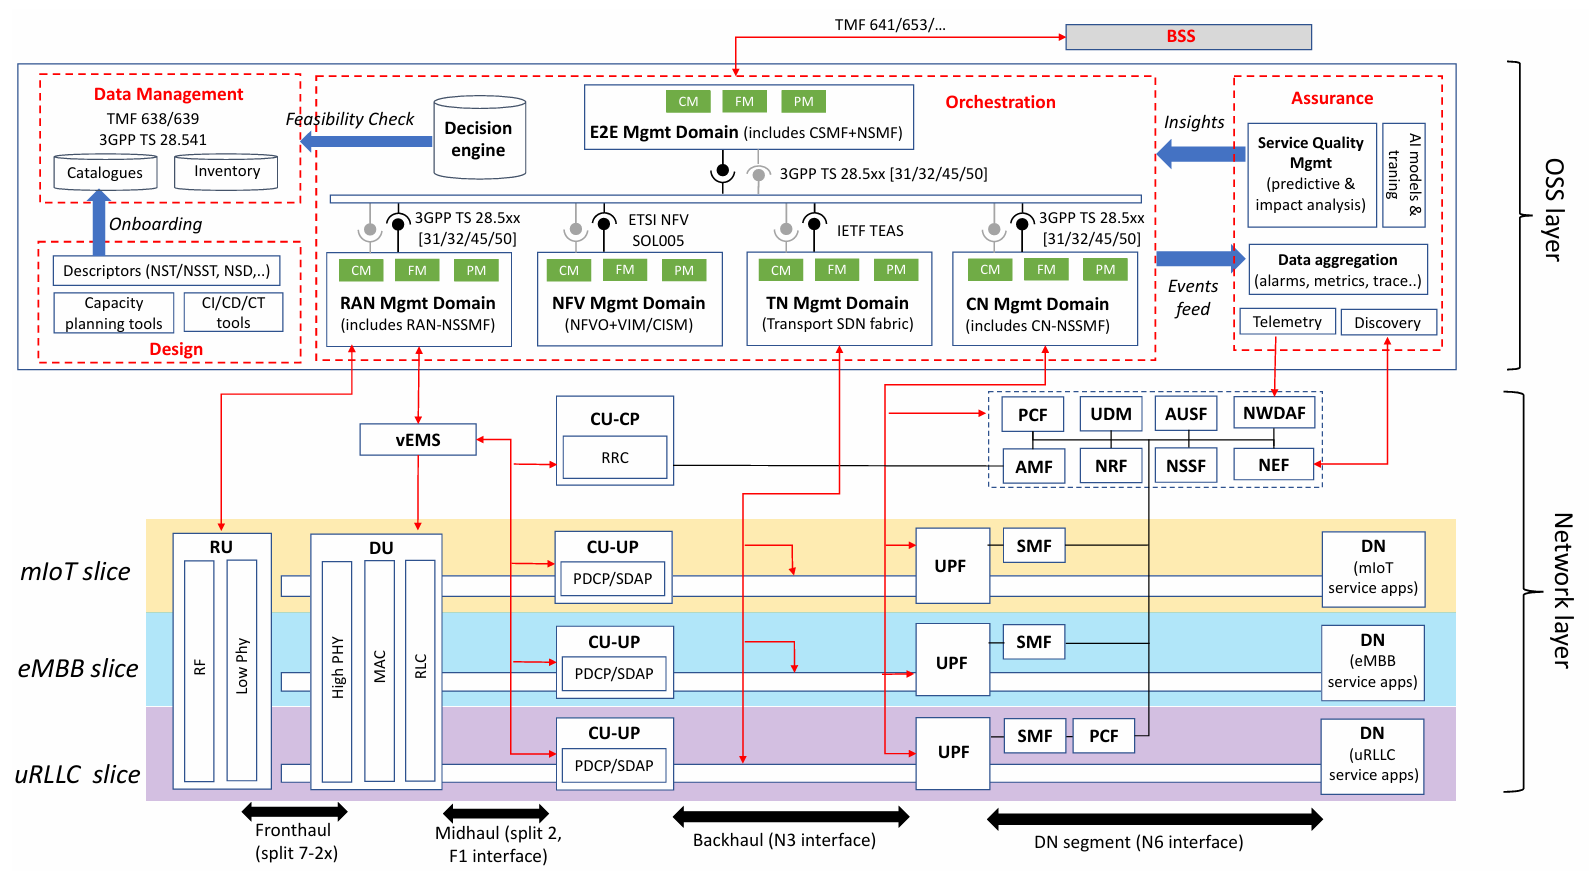
\includegraphics[width=0.8\linewidth]{img/2.1.1-three-slicing.png}
\caption{跨網域端到端網路切片架構示意圖 \cite{ordonez2021rollout}}
\label{fig:network_slicing}
\end{figure}

如圖 \ref{fig:network_slicing} 所示，各網域間之協作涉及複雜之參數映射與資源調配機制 \cite{ordonez2021rollout}。在典型之切片部署流程中，管理系統必須根據高階通訊服務之需求，將 E2E 之 SLA 指標拆解並下發至各網域之子網管理功能。具體而言，RAN 網域負責執行無線資源管理（RRM）與實體資源塊比率（PRB Ratio）之動態調度，以因應無線環境之瞬時變化；而 Core 網域則專注於會話管理與 5G QoS 標識符（5QI）之映射，確保數據流在用戶平面獲得預期之服務品質處理 \cite{nahum2025intent}。

儘管完整的 E2E 切片範疇包含負責中後傳連接之 TN 網域，本研究之實作範疇聚焦於 RAN 與 Core 之自動化編排。透過將 TN 配置視為既定之基礎設施，本研究得以排除傳輸層之變數，進而精確驗證意圖驅動架構在關鍵網元間之協調效能與參數轉譯之準確性。這種跨網域之協同運作，不僅是實現宣告式管理之基礎，更是達成閉環控制管道之關鍵技術門檻。


\subsection{電信雲化環境下之虛擬化基礎設施編排}
ETSI NFV-MANO（Management and Orchestration）框架為電信等級之虛擬化網路功能（Virtualized Network Function, VNF）提供了標準化之管理與編排架構 \cite{etsi_nfv_mano}。根據 ETSI GS NFV 006 規範，此架構旨在實現網路功能軟體與底層硬體資源之解耦，從而提升電信網路之服務靈活性與營運效率。

如圖 \ref{fig:etsi_nfv_arch} 所示，NFV 體系架構由三大核心領域構成：
\begin{itemize}
\item \textbf{NFV 管理與編排（NFV-MANO）}：包含 NFV 編排器（NFVO）、VNF 管理器（VNFM）與虛擬化基礎設施管理器（VIM）。其中 NFVO 負責網路服務（Network Service, NS）之全生命週期管理與資源編排；VNFM 負責 VNF 實例之生命週期管理；VIM 則負責對網路功能虛擬化基礎設施（NFVI）中之計算、存儲與網路資源進行控制與配給。
\item \textbf{VNF 與網元管理器（Element Manager, EM）}：VNF 為網路功能之軟體實作；EM 則負責 VNF 應用層面之配置、故障監測與性能管理。
\item \textbf{NFV 基礎設施（NFV Infrastructure, NFVI）}：涵蓋實體硬體資源與虛擬化層，為 VNF 之運行提供必要之計算能力、存儲空間與網路連通性。
\end{itemize}

該架構定義了多個關鍵之標準參考點（Reference Points），例如銜接 OSS/BSS 與 NFVO 之 Os-Ma-nfvo、協調 NFVO 與 VNFM 之 Or-Vnfm，以及介接 VNFM 與 VIM 之 Vi-Vnfm。這些標準化介面確保了在多廠商（Multi-vendor）環境下組件間之互操作性。透過軟硬體解耦與資源池化，NFV-MANO 支援了切片架構所需之動態資源配給與邏輯隔離，這與本研究之意圖驅動編排架構在資源層面之自動化調控需求緊密銜接 \cite{antonakoglou2025camino}。

\begin{figure}[H]
\centering
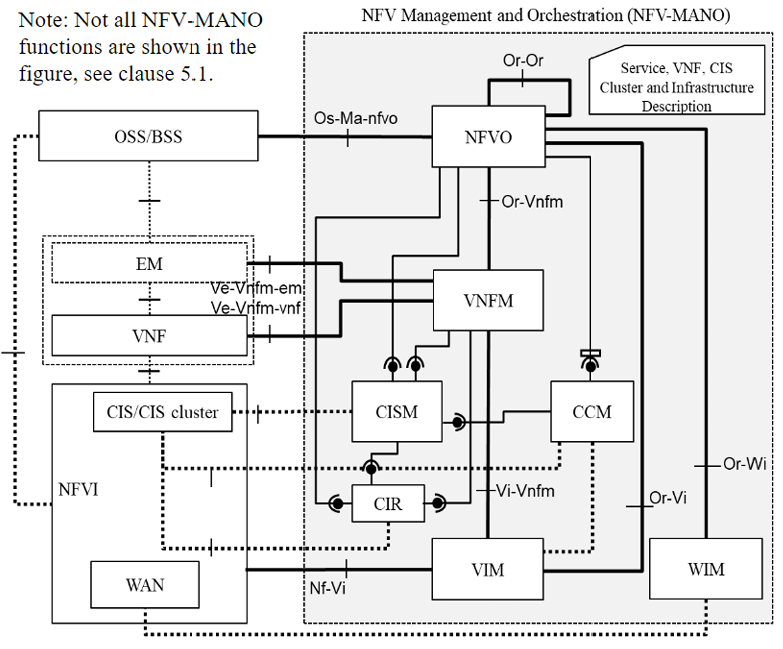
\includegraphics[width=0.8\linewidth]{img/2.1.3-ETSI-GS-NFV-006.png}
\caption{ETSI GS NFV 006 標準化架構與參考點定義示意圖 \cite{etsi_nfv_mano}}
\label{fig:etsi_nfv_arch}
\end{figure}


\subsection{服務化管理架構與網路切片編排機制}

在 5G 及其演進網路中，網路切片之管理與編排已全面轉向服務化管理架構（Service-Based Management Architecture, SBMA）。根據 3GPP TS 28.533 規範，管理系統不再依賴傳統之點對點命令式介面，而是透過管理服務（Management Service, MnS）之生產與消費機制進行交互。此範式將管理能力抽象化為靈活的服務界面，是達成網路自動化運維的核心基礎。

如圖 \ref{fig:mns_interaction} 所示，MnS 的交互呈現階層化的生產者（Producer）與消費者（Consumer）關係。在此模型中，最上層之 MnS Consumer（如 OSS/BSS）透過「網路與網路切片管理服務」下發意圖，而各管理功能則根據其職責提供對應的服務。

\begin{figure}[H]
\centering
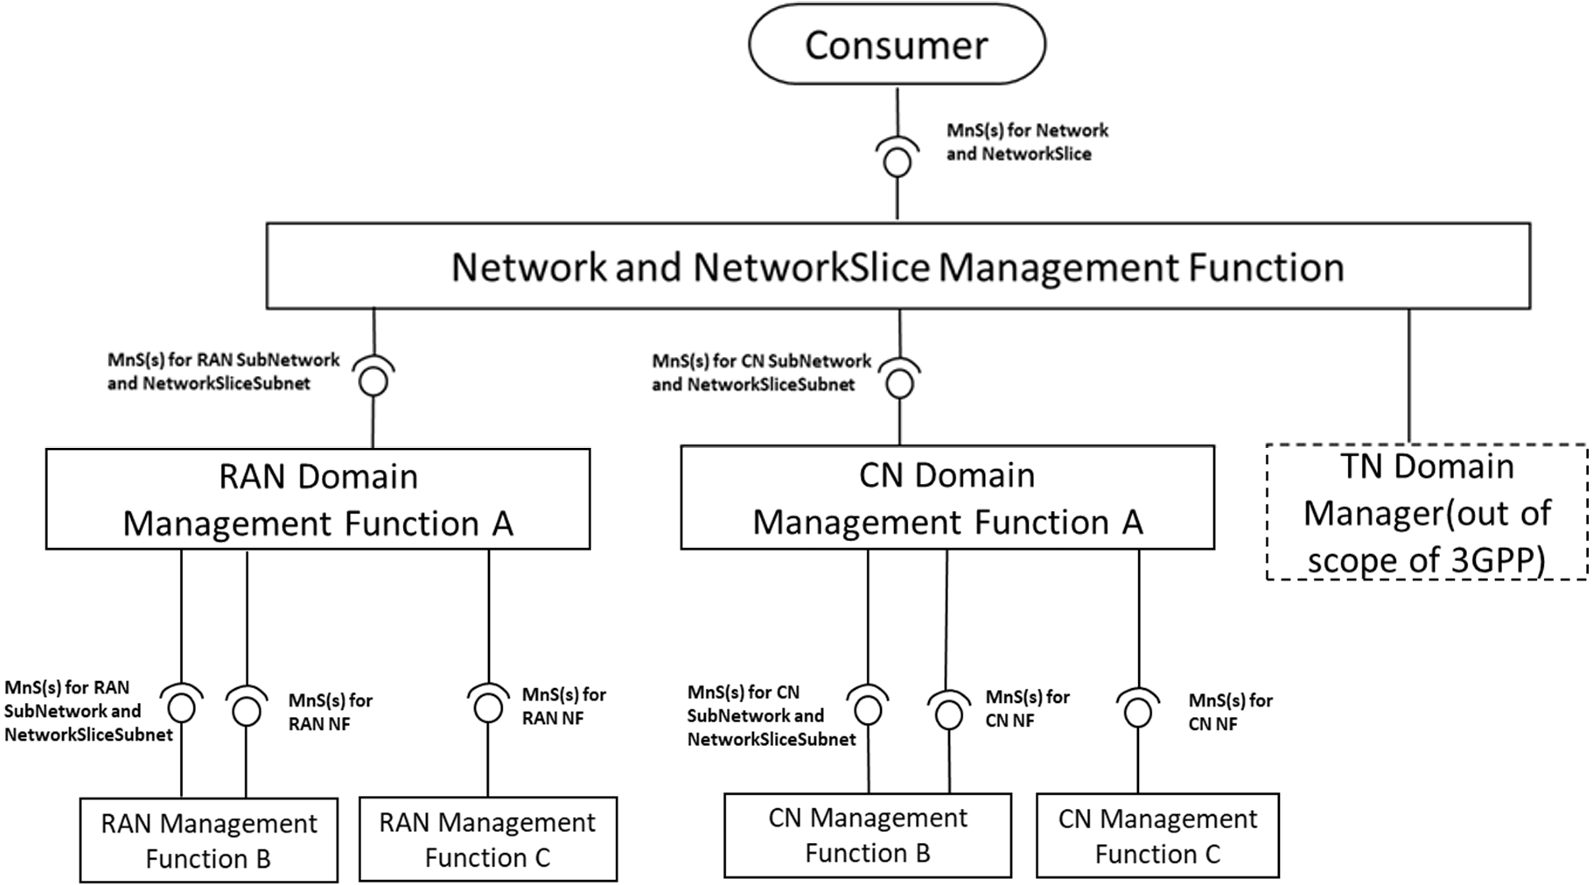
\includegraphics[width=0.8\linewidth]{img/2.1.4-MnS.png}
\caption{3 \cite{3gpp_ts28533}GPP 管理服務（MnS）之階層化交互模型}
\label{fig:mns_interaction}
\end{figure}

此交互範式揭示了管理功能在不同層級間的解耦邏輯：
\begin{itemize}
\item \textbf{能力抽象化}：MnS Producer（如各網域管理功能）向外暴露特定的管理能力，而 Consumer 僅需關注服務功能，無需介入底層網域之特定技術實現。
\item \textbf{階層化協調}：端到端（E2E）管理功能作為子網域服務的消費者，負責協調無線存取網（RAN）與核心網（CN）之資源，實現跨域之業務邏輯編排。
\end{itemize}

在實務部署中，此一服務化範式具體化為由網路切片管理功能（Network Slice Management Function, NSMF）統籌全局，並與各子網管理功能（Network Slice Subnet Management Function, NSSMF）協同運作之階層體系。

\begin{figure}[H]
\centering
\includegraphics[width=0.8\linewidth]{img/2.1.4-NSSMF.png \cite{3gpp_ts28533}}
\caption{3GPP 網路切片管理功能（NSMF/NSSMF）階層架構圖}
\label{fig:3gpp_management_hierarchy}
\end{figure}

如圖 \ref{fig:3gpp_management_hierarchy} 所示，NSMF 負責 NSI 之全生命週期管理。當 NSMF 接收到意圖請求後，會將業務層級之 SLA 轉譯為各子網域之技術規格。在雲原生電信環境中，此架構與 ETSI 之雲原生編排體系深度對應，分為以下職能層級：
\begin{itemize}
\item \textbf{意圖編排與協調層（NSMF / Intent Handler）}：作為系統大腦，負責消費意圖管理服務，將抽象期望解析為網域配置需求。
\item \textbf{配置管理服務框架（Provisioning MnS Framework）}：扮演雲原生網路功能編排器（Cloud-Native NFVO）之角色，負責套件（Package）之版本控制與發布。透過非同步機制，NSMF 得以將子網設定下發至儲存庫，無需直接調用底層介面。
\item \textbf{網域調和與執行層（NSSMF / VNFM）}：各網域之 Operator 實質承擔 NSSMF 職責，配合容器基礎設施服務管理（CISM）代理執行宣告式狀態同步，將期望狀態落實於實體網路功能（NFs）中。
\end{itemize}

此種基於 SBMA 與宣告式套件之編排範式，成功將跨域協調邏輯與領域特定實作解耦，為本研究實作之跨域閉環控制提供了核心之理論支撐。
\subsection{意圖驅動管理之核心原理與工作流程}

根據 3GPP TS 28.312 規範，意圖驅動管理代表了從傳統命令式配置轉向「以目標為導向（Outcome-oriented）」管理 \cite{3gpp_ts28312}範式之轉變。在此模型下，意圖被定義為對網路期望狀態之宣告式描述，系統需具備自主轉譯與執行之能力，以屏蔽底層網路之技術複雜性。

為了釐清意圖在不同管理層級間的傳遞關係，3GPP 定義了明確的角色模型與服務邊界。如圖 \ref{fig:intent_role_model} 所示，意圖的交互涵蓋了從通訊服務客戶（Communication Service Customer, CSC）到網路營運商（Network Operator, NOP）的多層級對映。

\begin{figure}[H]
\centering
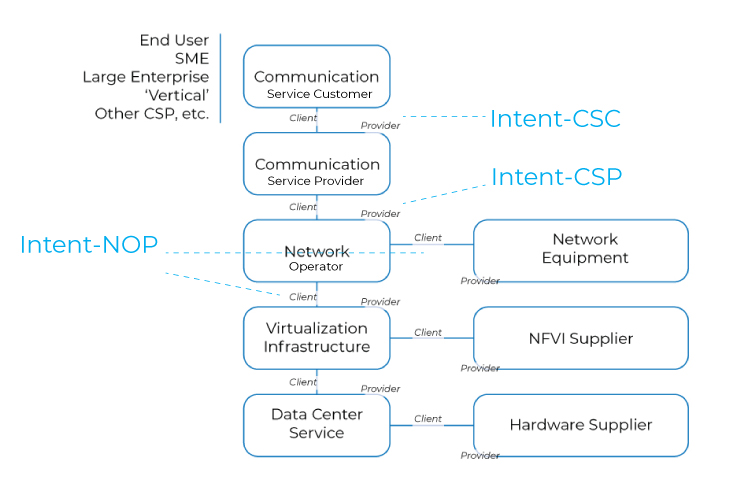
\includegraphics[width=0.8\linewidth]{img/2.1.4-intent-MNS.jpg}
\caption{意圖驅動管理之角色模型與層級對映圖 \cite{3gpp_ts28312}}
\label{fig:intent_role_model}
\end{figure}

在該模型中，不同角色所下發的意圖具備不同的抽象程度與業務目標。該規範將意圖進一步分為以下三類：

\begin{itemize}
\item \textbf{交付意圖（Delivery Intent）}：側重於網路資源或服務之初始佈署。例如：要求「於特定地理區域內部署具備 eMBB 能力之網路切片實例」。
\item \textbf{保障意圖（Assurance Intent）}：側重於維持特定之服務品質目標，以應對網路環境之動態變化。例如：要求「確保 URLLC 切片之端到端延遲恆低於 10 毫秒」。
\item \textbf{優化意圖（Optimization Intent）}：側重於在滿足既有需求之前提下，極大化資源利用效率。例如：要求「在維持現有流量負載之同時，將無線電能量損耗降至最低」。
\end{itemize}

本研究所實作之 \texttt{E2EQoSIntent} 主要歸類為\textbf{保障意圖}，其核心價值在於透過意圖管理服務（Intent Management MnS）定義高階之 SLA 期望，並由自動化編排管道維持這些性能指標。標準之意圖驅動工作流程可具體對應至本研究之系統設計，達成從抽象需求到實體配置之閉環控制：

\begin{enumerate}
\item \textbf{意圖提取（Extraction）}：\textbf{E2E Orchestrator (Intent Handler)} 透過 \textbf{Intent Management MnS 介面} 持續監聽由 \textbf{MnS Consumer (Intent Owner)} 提交之 \texttt{E2EQoSIntent} 自定義資源，將其宣告式期望提取為內部狀態模型。
\item \textbf{意圖轉譯（Translation）}：扮演 \textbf{NSMF} 職責之編排器內建轉譯引擎，將抽象 SLA 映射為領域參數。具體而言，系統根據映射表將延遲需求轉化為 Core 網域之 5QI 值，並根據資源佔比需求決定 RAN 網域之 PRB Ratio 與優先權配置。
\item \textbf{意圖執行（Execution）}：轉譯後之指令經由 \textbf{配置管理服務框架（Provisioning MnS Framework）} 下發。針對 RAN 網域，系統發起套件變更與發布工作流；針對 Core 網域，則同步驅動 \textbf{Core NSSMF} 完成 QoS 配置。
\item \textbf{閉環監測與回報（Monitoring and Reporting）}：編排器在配置生效後，會自動更新資源之狀態（Status）欄位，回報當前之達成狀態（Fulfillment State）。此機制確保 MnS Consumer 能即時驗證意圖是否已成功落實於底層網路功能（NFs）中。
\end{enumerate}

\section{雲原生電信架構與開發平台}

\subsection{5G Core 與 RAN 之開放性實作}

本研究之實驗平台建立於開源之 5G 行動通訊系統基礎之上，旨在提供一個具備高度透明度且可自定義之端到端驗證環境。透過整合核心網與無線存取網之開源實作，本系統得以精確控制從意圖轉譯至底層資源分配的完整流程。

\textbf{1. free5GC 核心網架構設計} \
free5GC \cite{free5gc} 係首個基於 3GPP Release 15 規範實作之開源 5G Core 專案，其核心設計採納了服務化架構（Service-Based Architecture, SBA）。如圖 \ref{fig:3gpp_r15_arch} 所示，SBA 透過統一之服務基礎設施（Service Bus），使各個網路功能（Network Function, NF）得以解耦為服務生產者與消費者進行溝通。free5GC 充分利用 Go 語言之併發處理能力與記憶體管理優勢，實作了包含控制面與用戶面分離（CUPS）之完整協議棧。

\begin{figure}[H]
\centering
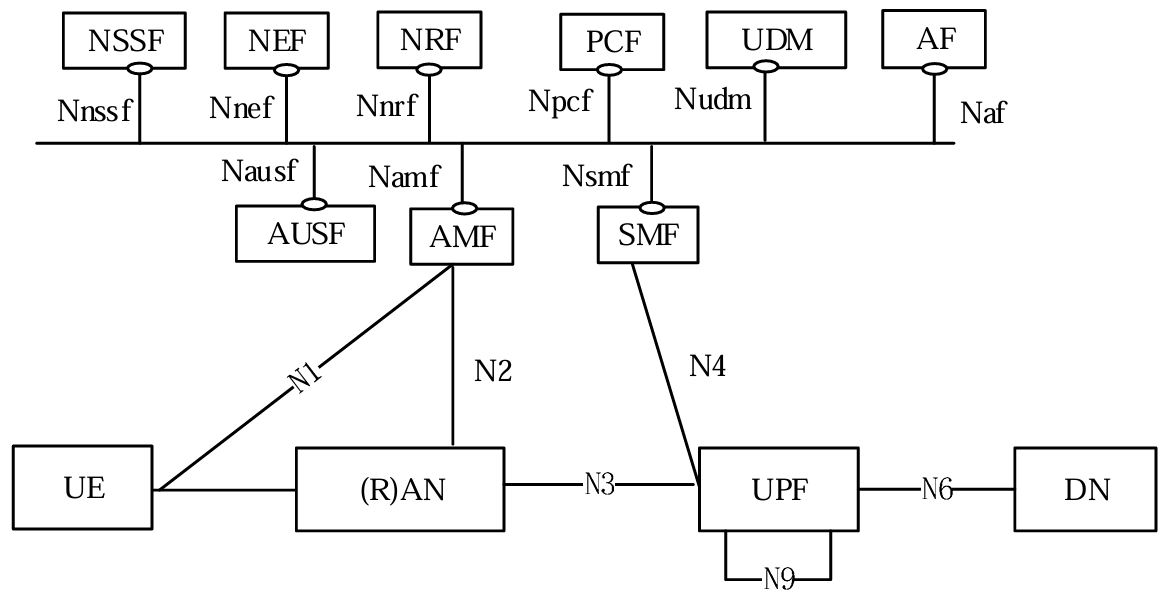
\includegraphics[wi \cite{3gpp_ts23501}dth=0.8\linewidth]{img/2.2.1-r15-arch.png}
\caption{3GPP Release 15 服務化架構（SBA）示意圖}
\label{fig:3gpp_r15_arch}
\end{figure}

在網路切片之運作脈絡中，free5GC 之各個 NF 實質上扮演了核心網子網管理（Core NSSMF）之執行實體，其職能如下：
\begin{itemize}
\item \textbf{AMF（Access and Mobility Management Function）}：作為 UE 接入之單一入口，負責處理註冊信令，並根據網路切片選取輔助資訊（NSSAI）判定 UE 請求之切片合法性。
\item \textbf{SMF（Session Management Function）}：負責會話管理，針對不同切片建立獨立之 PDU 會話，並根據意圖轉譯後之 QoS 參數配置 UPF 轉發路徑。
\item \textbf{UPF（User Plane Function）}：執行數據封包之路由與轉發，是實作切片流量隔離之實體平面，確保不同服務等級之數據流在用戶平面互不干擾。
\item \textbf{NSSF（Network Slice Selection Function）}：為特定之 UE 選擇最適當之切片實例，是 Core 網域內進行切片決策與導向之核心組件。
\end{itemize}

\textbf{2. srsRAN 無線存取網架構設計} \
srsRAN \cite{srsran} 是一套完整之軟體定義無線電（SDR）解決方案。在其最新演進之 5G 架構中，srsRAN 遵循了 O-RAN 聯盟定義之功能拆分規範，將傳統基地台解耦。如圖 \ref{fig:srsran_arch} 所示，srsRAN 實作了包含 O-CU 與 O-DU 在內之組件，並支持標準化之 E1 與 F1 介面通訊。此種架構支持高效能處理，其高度參數化之特性使其成為研究 RAN 切片與動態資源調度之理想工具 \cite{nahum2025intent}。

\begin{figure}[H]
\centering \cite{srsran_oran_gnb_doc}
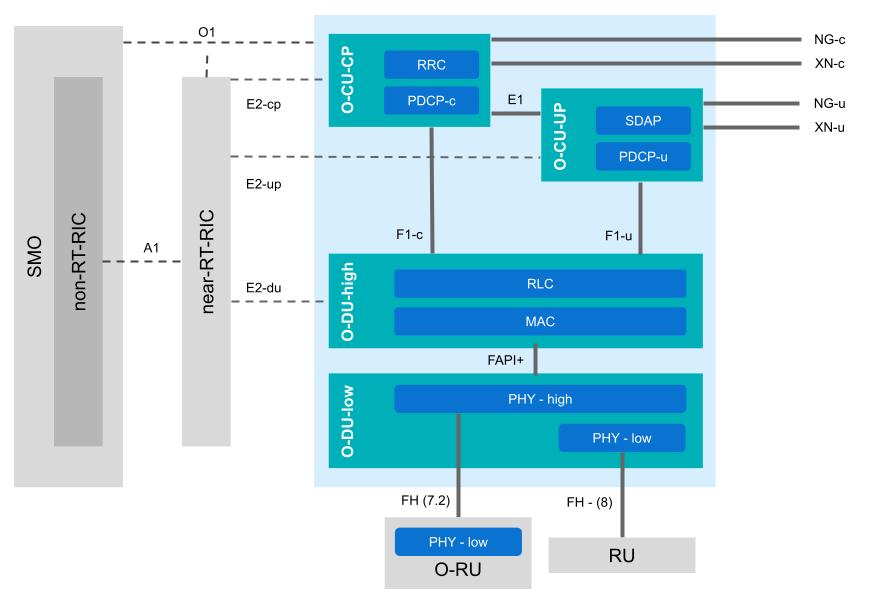
\includegraphics[width=0.8\linewidth]{img/2.2.1-srsRAN-arch.jpg}
\caption{srsRAN 遵循 O-RAN 規範之解耦架構示意圖}
\label{fig:srsran_arch}
\end{figure}

針對端到端切片之自動化配置，srsRAN 各組件之角色與功能定義如下：
\begin{itemize}
\item \textbf{O-CU-CP（Centralized Unit - Control Plane）}：處理無線資源控制（RRC）與 PDCP 控制面信令，並與 Core 進行 NG-c 對接，是 RAN 網域之控制核心。
\item \textbf{O-CU-UP（Centralized Unit - User Plane）}：處理服務數據適應協議（SDAP）與用戶面 PDCP，負責將用戶面數據（NG-u）映射至特定之 QoS 流。
\item \textbf{O-DU（Distributed Unit）}：涵蓋 RLC、MAC 與高層實體層（High-PHY）。DU 是本研究實施資源隔離之核心場域，其透過 MAC 層執行實體資源塊比率（PRB Ratio）分配與調度優先權管理，直接決定不同切片之服務表現 \cite{nahum2025intent, tran2024ina}。
\end{itemize}

透過 free5GC 與 srsRAN 之深度整合，本研究構建了一個橫跨控制面意圖轉譯與用戶面資源實施之完整實驗床，為驗證宣告式編排流程提供了必要之功能完備性。

\subsection{Kubernetes 平台架構與 Operator 開發模式}

Kubernetes 作為雲原生環境之核心編排平台，其架構優勢在於定義了一套標準化的聲明式（Declarative）管理範式。其底層設計遵循 Kubernetes 資源模型（KRM），該模型規定了所有資源對象均需透過統一的 API 規範進行定義，並將「期望狀態（Desired State）」持久化於 etcd 數據庫中 \cite{antonakoglou2025camino}。這種將配置與邏輯分離的設計，使得複雜網路功能的部署得以轉化為對結構化數據的操作。

為了因應電信領域之特殊需求，Kubernetes 提供了自定義資源定義（Custom Resource Definition, CRD）機制，允許開發者擴展原生 API 伺服器之功能。透過 CRD，系統得以定義如網路切片意圖或網元配置等特定領域的數據模型，並將其實例化為自定義資源（Custom Resource, CR） \cite{tran2024ina}。這種擴展性確保了電信網路的領域知識能無縫整合至雲原生生態系中，使網路服務之編排與一般應用程式之管理具備一致性的操作界面。

Operator 模式則是落實上述聲明式管理之核心技術路徑。其運作邏輯基於調和迴圈（Reconciliation Loop），由控制器（Controller）持續監控特定 CR 之狀態變更 \cite{ghosh2025performance}。當控制器偵測到 etcd 中儲存之「期望狀態」與底層系統之「實際狀態（Actual State）」存在差異時，將觸發預設之轉譯與執行邏輯，自動執行必要的配置操作以消除偏差。

一個典型的 Kubernetes 資料流轉過程如下：首先，上層應用透過 API 伺服器提交 CR，並由 API 伺服器完成架構驗證與持久化；隨後，負責該資源之 Operator 透過事件驅動（Event-driven）機制獲知變更，並於調和迴圈中執行資源渲染、參數轉譯或南向介面調用等任務 \cite{antonakoglou2025camino}。最終，Operator 將執行結果更新至資源之狀態（Status）欄位，完成閉環管理。這種機制不僅賦予了系統自動化部署之能力，更提供了關鍵的自癒（Self-healing）特性，是實作意圖驅動管理系統之理想軟體開發範式。

\subsection{宣告式自動化與 Nephio 編排流程}

Nephio \cite{nephio} 透過「配置即數據（Configuration as Data, CaD）」範式，將電信等級之複雜配置轉化為可受 Kubernetes 管理之標準化數據對象。其核心價值在於建立一套跨叢集之宣告式自動化管道，達成從藍圖（Blueprint）定義到實體網路功能（NF）部署之閉環管理。

\be \cite{nephio_level2_arch_image}gin{figure}[H]
\centering
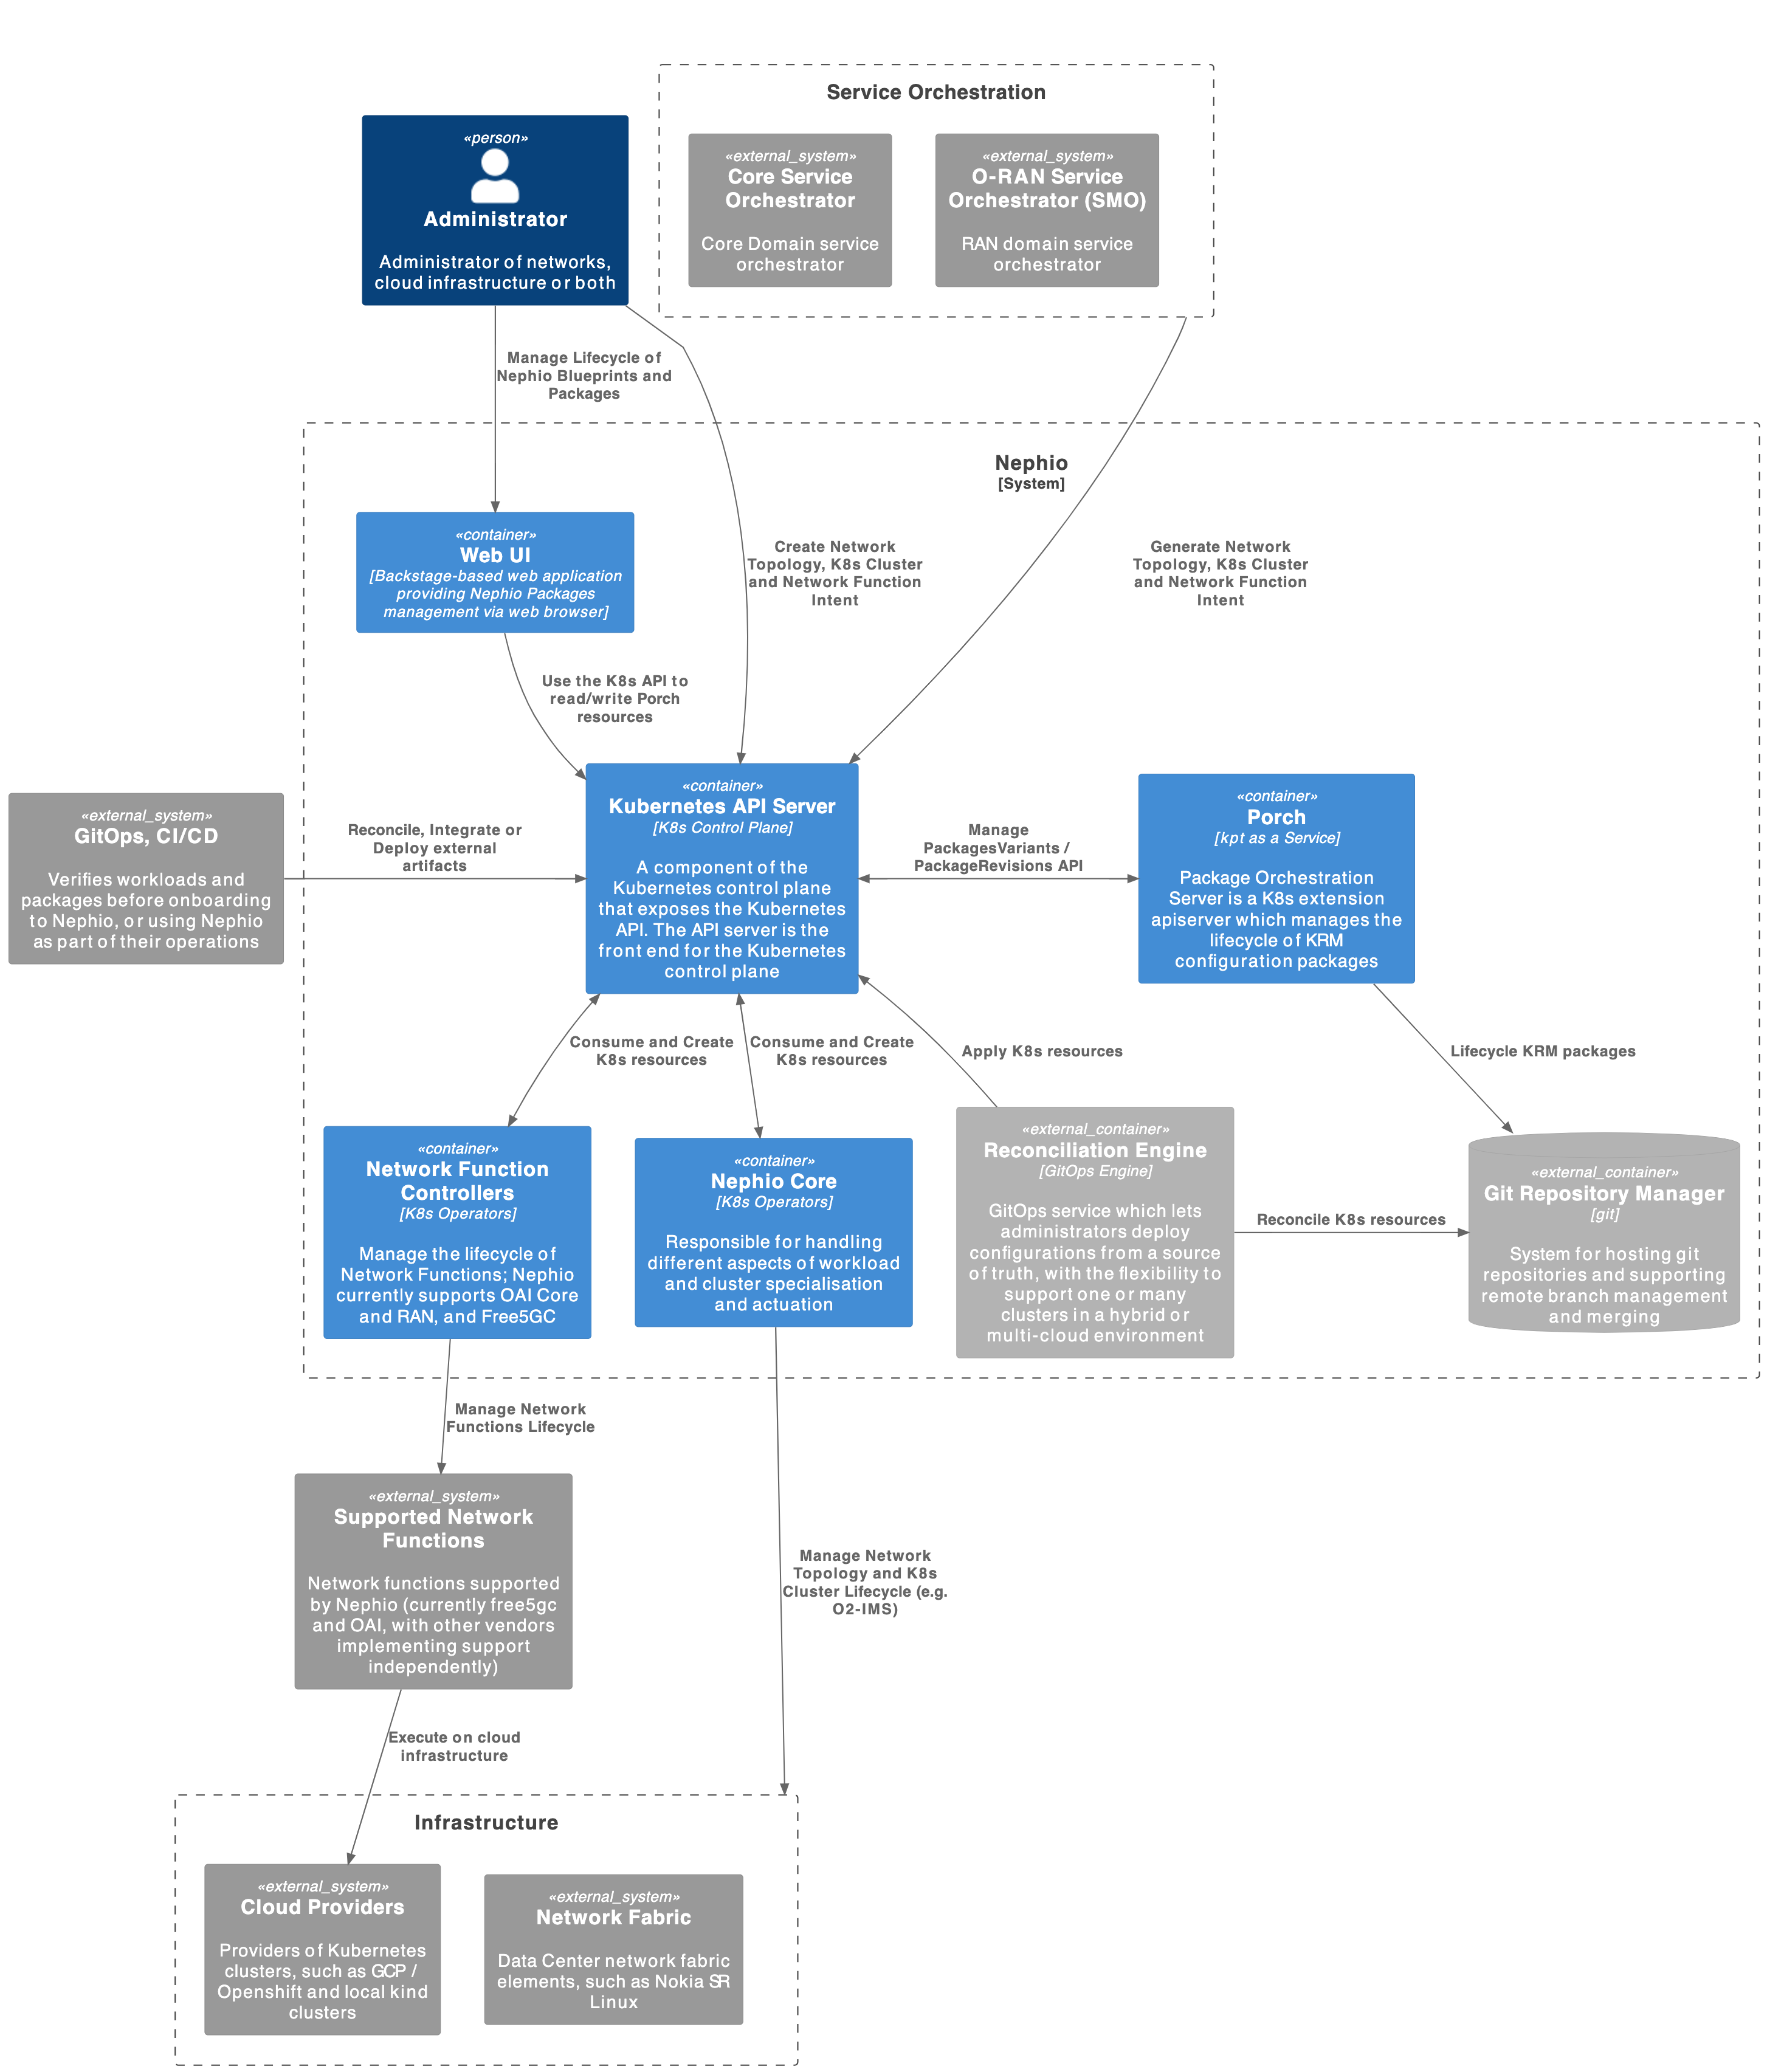
\includegraphics[width=0.8\linewidth]{img/2.2.3-nephio-workflow.png}
\caption{Nephio 宣告式編排與套件自動化工作流架構圖}
\label{fig:nephio_workflow}
\end{figure}

如圖 \ref{fig:nephio_workflow} 所示，完整之 Nephio 管理工作流程橫跨管理叢集（Management Cluster）與工作負載叢集（Workload Cluster），其運作機制具體對應至 3GPP 配置管理服務框架（Provisioning MnS Framework）與雲原生網路功能編排器（Cloud-Native NFVO）之職能：

\begin{enumerate}
\item \textbf{藍圖定義與套件初始化}：開發者首先將包含 KRM 資源模板之套件定義為藍圖。此藍圖定義了特定網路功能之基本配置結構，作為生成各網元實體配置之基礎來源。
\item \textbf{套件生命週期管理（Porch）}：於管理叢集中，編排器透過 Porch 套件管理系統執行複製操作，從藍圖建立針對特定網元之套件修訂版本（PackageRevision）草案。隨後，系統於變更（Mutate）階段注入由 NSMF 轉譯後之領域參數。完成變更後，依序執行提議（Propose）與核准（Approve）程序，將套件狀態轉為「已發布（Published）」。
\item \textbf{發布與存儲}：獲准發布之套件會被推送至部署儲存庫（Git Repository Manager），作為整個系統中對於配置狀態之單一事實來源（Single Source of Truth）。
\item \textbf{自動化同步（ConfigSync）}：位於工作負載叢集之配置同步組件（又稱 CISM Agent）持續監控儲存庫之變更。一旦偵測到版本更新，便會自動將 KRM 資源對象拉取至叢集內部命名空間，將「期望狀態」同步至實際運行環境中。
\item \textbf{Operator 調和與實體渲染}：工作負載叢集內之 Operator（職司 NSSMF/VNFM）監聽到同步後之自定義資源（CR）。Operator 隨即執行調和迴圈，將 KRM 參數動態映射並產生底層網元所需之實體設定檔案，最終驅動 Pod 啟動服務，完成從宣告式意圖到實體配置生效之完整鏈結。
\end{enumerate}

這種架構將原本碎片化之手動配置流程轉化為標準化、版本化且具備自癒能力之自動化管道，有效提升了跨域配置之準確性與一致性。
% \subsection{宣告式自動化與 Nephio 編排流程}
% Nephio \cite{nephio} 透過「配置即數據（Configuration as Data, CaD）」範式，將電信等級之複雜配置轉化為可受 Kubernetes 管理之標準化數據對象。其核心價值在於建立一套跨叢集之宣告式自動化管道，達成從藍圖（Blueprint）定義到實體網路功能（Network Function, NF）部署之閉環管理。

% 完整之 Nephio 管理工作流程橫跨管理叢集（Management Cluster）與工作負載叢集（Workload Cluster），其運作機制如下：

% \begin{enumerate}
% \item \textbf{藍圖定義與套件初始化}：開發者首先將包含 KRM（Kubernetes Resource Model）資源模板之套件定義為藍圖。此藍圖定義了特定網路功能之基本配置結構，作為生成各網元實體配置之基礎架構來源。
% \item \textbf{套件生命週期管理}：於管理叢集中，編排器透過 Porch 套件管理系統執行複製操作，從藍圖建立針對特定網元之套件修訂版本（PackageRevision）草案。隨後，系統於變更（Mutate）階段注入經由意圖轉譯後之領域參數。完成變更後，依序執行提議（Propose）與核准（Approve）程序，將套件狀態轉為「已發布（Published）」。
% \item \textbf{發布與存儲}：獲准發布之套件會被推送至部署儲存庫（如 Git 儲存庫或 OCI 映像倉庫），作為整個系統中對於配置狀態之單一事實來源。
% \item \textbf{自動化同步}：位於工作負載叢集之配置同步組件（ConfigSync）持續監控儲存庫之變更。一旦偵測到版本更新，便會自動將 KRM 資源對象拉取至叢集內部命名空間，將「期望狀態」同步至實際運行環境中。
% \item \textbf{Operator 調和與實體渲染}：工作負載叢集內之 Operator 監聽到同步後之自定義資源（Custom Resource, CR）。Operator 隨即執行調和迴圈，將 KRM 參數動態映射並產生底層網元所需之實體設定檔案。這些設定通常以原生 Kubernetes 資源之形式存在，最終驅動 Pod 啟動服務，完成從宣告式意圖到實體配置生效之完整鏈結。
% \end{enumerate}

% 這種架構將原本碎片化之手動配置流程轉化為標準化、版本化且具備自癒能力之自動化管道，有效提升了跨域配置之準確性與一致性。
% \begin{figure}[H]
%     \centering
%     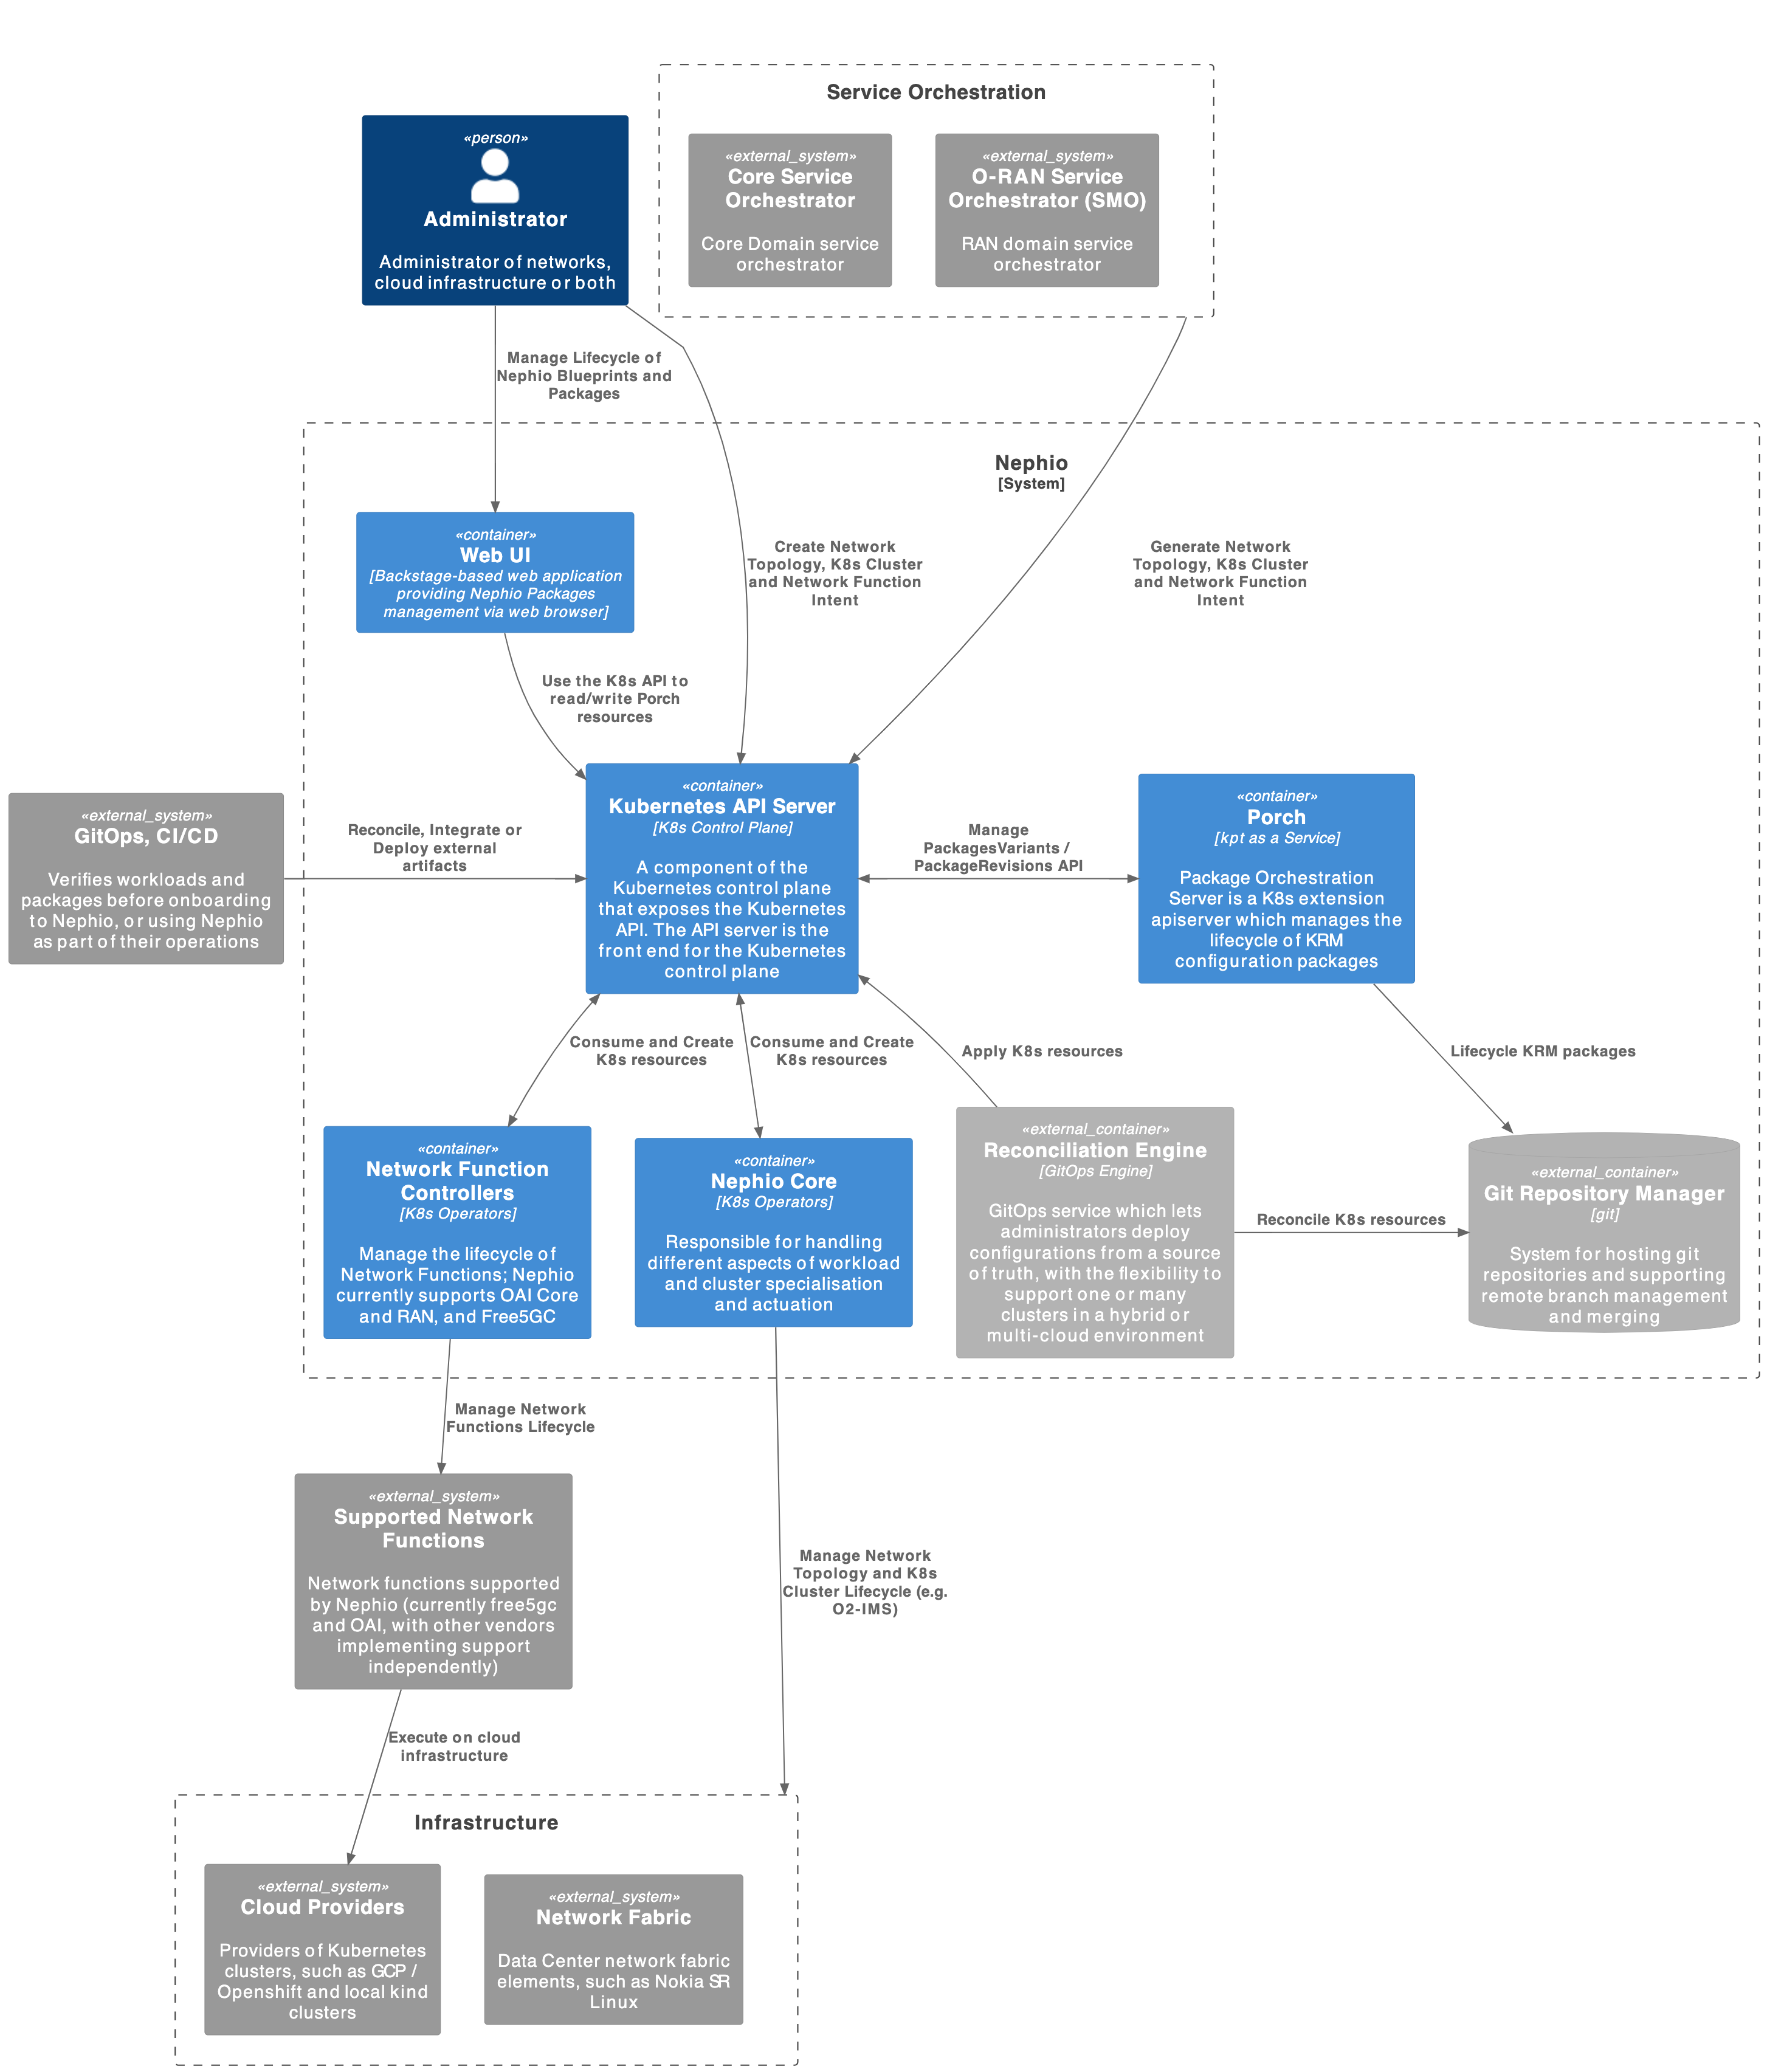
\includegraphics[width=0.8\linewidth]{img/2.2.3-nephio-workflow.png}
%     \caption{Enter Caption}
%     \label{fig:placeholder}
% \end{figure}

\section{意圖驅動網路管理與自動化編排之文獻回顧}

\subsection{意圖驅動自動化框架之發展現況}
近年來，學術界針對意圖驅動管理與端到端（E2E）網路切片之結合展開了深入研究。Chirivella-Perez 等人 \cite{chirivella2023e2e} 提出了一套適用於 5G 多租戶網路的 E2E 切片管理框架，強調了在異質網域間進行動態資源協調的必要性，以滿足租戶間的隔離需求。與此同時，針對關鍵任務之服務保障，Martini 等人 \cite{martini2023intent} 探討了在意圖型網路中如何透過定義明確的上下文與設計模型，為垂直產業提供具備性能保障（Assurance）的切片服務。這些研究共同奠定了意圖驅動架構在理論模型與初步驗證上的基礎。

在此基礎上，後續研究進一步結合雲原生技術以優化編排之自動化水準。INA-Infra \cite{tran2024ina} 與 CAMINO \cite{antonakoglou2025camino} 代表了當前的技術演進方向，其利用 Nephio 專案與「配置即數據（CaD）」範式，實作了跨多邊緣基礎設施之零接觸供應與自動化服務管理。針對宣告式管道之效率，Ghosh 等人 \cite{ghosh2025performance} 進一步量化分析了包括 ConfigSync 在內之 GitOps 工具於意圖型場景下之處理延遲。此外，如 Nahum 等人 \cite{nahum2025intent} 之研究則專注於無線電資源調度之優化，探索利用機器學習技術於 RAN 切片中精確滿足多樣化之 SLA 要求。從整體架構、保障機制到特定網元之調度優化，這些文獻共同建構了當前意圖驅動網路編排之技術圖譜。

\subsection{現有文獻之研究缺口與技術挑戰}

儘管前述研究在意圖驅動框架與切片管理上取得了初步進展，但在邁向高度自動化的 6G 演進過程中，仍存在顯著的技術缺口。首先，在意圖轉譯（Intent Translation）之細節實作上，雖然 3GPP TS 28.312 提供了規範指引，但現有研究如 CAMINO \cite{antonakoglou2025camino} 與 INA-Infra \cite{tran2024ina} 對於如何將抽象的服務期望映射至底層異質參數的過程描述較為宏觀，缺乏一套具體的轉譯引擎，能精確且同時將高階 SLA 需求轉化為 Core 網域之 5QI 與 RAN 網域之 PRB Ratio 資源調度策略。這種語意轉譯能力的缺失，導致上層應用程式（rApp）的意圖難以直接落實於物理資源層面。

其次，跨網域之南向介面整合面臨異質技術棧之同步難題。Martini 等人 \cite{martini2023intent} 與 Chirivella-Perez 等人 \cite{chirivella2023e2e} 雖討論了多租戶服務保障之重要性，但其系統實作往往側重於單一控制平面之邏輯，未能解決當前雲原生電信環境中混合式介面之編排困境。具體而言，如何將基於 GitOps 流程之 RAN 配置套件變更，與基於 REST API 之 Core 使用者註冊與 QoS 配置，整合進單一之意圖調和週期（Reconciliation Loop）內，在現有文獻中仍缺乏有效的解決方案。此外，Nahum 等人 \cite{nahum2025intent} 之研究雖然深入探討了 RAN 內部之調度優化，卻缺乏與管理平面之聯動機制，導致無線電資源之分配難以與 Core 之會話狀態達成即時之一致性。

最後，現有文獻之驗證環境呈現高度碎片化之趨勢。雖然 Ghosh 等人 \cite{ghosh2025performance} 評估了 GitOps 工具之處理效能，但相關研究多將網路功能（NF）與使用者設備（UE）之部署視為獨立事件，缺乏標準化之組件化方案。特別是對於如 \texttt{srsue} 等模擬工具，現有架構多缺乏與 Kubernetes 生命周期管理深度整合之封裝，使其難以被納入端到端之自動化驗證管道中。這種組件整合之缺失，不僅增加了實驗環境之配置複雜度，也限制了系統對於動態意圖變更之系統性量測能力。

\subsection{本研究對既有技術缺口之彌補}
本研究旨在填補上述文獻中之技術落差，設計並實作了一套基於 KRM 之宣告式 R1 介面與 E2E Intent Orchestrator。相較於現有研究，本系統不僅實作了具體的轉譯引擎以精確映射 SLA 至 5QI 與實施 RAN 資源隔離，更透過混合南向介面串接了 Nephio Porch 的 GitOps 工作流與 free5GC API，解決了跨域配置同步之難題 \cite{tran2024ina}。此外，本研究藉由 \texttt{srsran-helm} 方案將 srsue 封裝為標準化之應用組件，實現了從意圖提交到無線電資源生效之完整自動化管道。這種端到端的系統性整合，不僅驗證了意圖驅動管理之可行性，更為電信網路之自動化運維提供了一個具備實踐價值的參考架構。
